\chapter{Introduzione}  
La stima della profondità ha da sempre rappresentato un problema di notevole interesse. L'informazione sulla profondità è importante, ed in alcuni casi essenziale, per molteplici applicazioni pratiche della visione artificiale: guida autonoma, robotica, ricostruzione 3D e realtà aumentata sono soltanto alcune. \par
L'acquisizione delle geometrie tridimensionali di scene del mondo reale rappresenta da sempre un problema complesso, e gli strumenti sono stati accessibili soltanto in grosse compagnie e centri di ricerca. Nel corso degli anni, molte tecniche sono state sviluppate e nuovi dispositivi, dai costi più ridotti, sono stati introdotti nel mercato.\par
Le principali tecnologie per la percezione dell'ambiente sfruttano sensori ottici che catturano la luce visibile o infrarossa che viene riflessa dalla scena. Questo lavoro di tesi tratta due categorie di sensori in particolare, entrambi molto diffusi e accessibili: i sensori a visione stereoscopica e i sensori basati sul tempo di volo (Time-Of-Flight, ToF).\par
Nello stesso periodo, nel mondo della computer vision, il machine learning (e in particolare il deep learning) si è dimostrato uno strumento che ha permesso di ottenere risultati impensabili con altri metodi deterministici, in molti problemi ritenuti complessi, fino a superare le prestazioni umane. E proprio grazie al machine learning è stato possibile sviluppare sistemi efficaci per la ricostruzione delle informazioni catturate da diverse tipologie di sensori.

\section{Descrizione del progetto}
L'obiettivo del lavoro di questa tesi è lo sviluppo di un sistema di machine learning per la fusione dei dati tridimensionali forniti dai sensori, cercando di fornire una ricostruzione più accurata. La scelta dei sensori gioca perciò un ruolo fondamentale: le telecamere stereo e il sensore ToF tendono ad avere caratteristiche complementari, e la loro combinazione si è rivelata efficace negli ultimi anni. 

\section{Principi di funzionamento del sistema di acquisizione}
Il sistema di acquisizione è composto da una coppia di telecamere stereo e da un sensore Time-of-Flight disposti vicino. I due dispositivi catturano la stessa scena allo stesso istante.

\begin{figure}[ht]
    \centering
    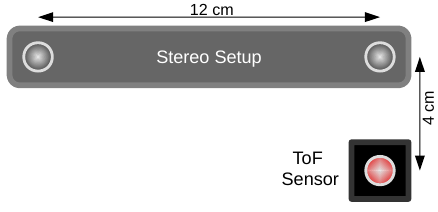
\includegraphics[width=0.5\columnwidth]{tof_stereo_acquisition_system}
    \caption[Sistema di acquisizione ToF-Stereo]{Rappresentazione del sistema di acquisizione ToF-Stereo. Il sensore ToF è posizionato sotto la telecamera di riferimento della coppia stereo \cite{realfusion}.}
\end{figure}

\subsection{Sistema di visione stereo}
Il sensore a visione stereoscopica consiste nell'acquisire due immagini bidimensionali da una coppia di telecamere allineate che inquadrano la stessa scena. Successivamente, in fase di post-processing realizzato via software, viene effettuata una operazione di calibrazione detta rettificazione con lo scopo di rendere complanari le due immagini e allineate sullo stesso asse \cite{rif1}. Lo stesso punto P dello spazio viene proiettato nel piano dell'immagine di ciascuna delle telecamere. I punti risultanti \(p_L\) e \(p_R\), detti \textit{omologhi}, hanno le stesse coordinate verticali, considerata la rettificazione dei sensori. Viene chiamata \textit{disparità} lo scostamento tra le coordinate orizzontali: \[d = u_L - u_R\] Tramite questo valore è possibile determinare la posizione del punto P nello spazio.\par
Uno dei principali vantaggi è il costo ridotto delle telecamere CCD o CMOS, facilmente accessibili nel mercato. Tale sensore è inoltre passivo, quindi può sfruttare l’illuminazione dell’ambiente. Ciò permette di essere utilizzato in ambienti esterni, al contrario di altri sensori che sfruttano
pattern proiettati con illuminatori. Inoltre può avere alte risoluzioni e una limitata quantità di rumore.\\
Lo svantaggio maggiore è la dipendenza dei risultati forniti da questi sensori dalla tessitura delle immagini utilizzata nel calcolo degli omologhi, ad esempio sono evidenti delle difficoltà nell'analisi di scene con pattern uniformi o ripetitivi. Pertanto essi presentano una robustezza solitamente limitata.

\begin{figure}[ht]
    \centering
    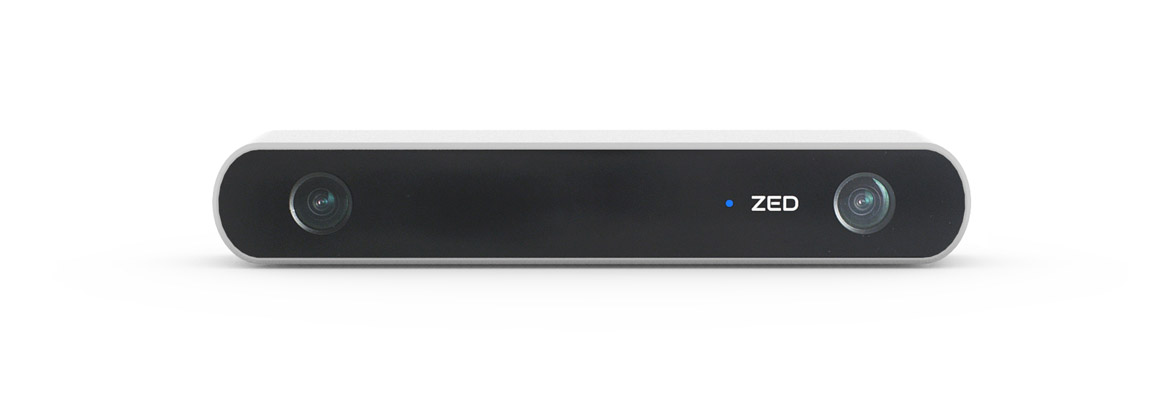
\includegraphics[width=0.5\columnwidth]{ZED}
    \caption[Sensore di visione stereo]{Sensore stereo ZED}
\end{figure}

\subsection{Sensore Time-Of-Flight}
Il sensore ToF determina le informazioni riguardo la profondità sulla base del fatto che le onde elettromagnetiche viaggiano alla velocità \(c\approx3\times 10^8[m/s]\). Il sensore emette un impulso luminoso (tipicamente infrarosso) il quale colpisce la scena e viene riflesso indietro. Viene dunque misurato il tempo $\tau$ che occorre al segnale luminoso per percorrere un tragitto pari al doppio della distanza dell'oggetto dalla telecamera $\rho$. La relazione che lega $\rho$ e $\tau$ è $$\rho=\frac{c\tau}{2}$$
Per misurare il tempo cercato e migliorare la risoluzione del sensore, l'impulso emesso è modulato secondo un segnale sinusoidale, così che anche l'eco abbia lo stesso andamento, ma
sfasato e attenuato in ampiezza.
\begin{figure}[ht]
    \centering
    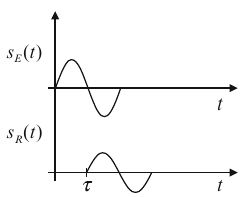
\includegraphics[width=0.4\columnwidth]{time-of-flight}
    \caption[Principio time-of-flight]{Segnale sinusoidale trasmesso e corrispondente segnale ricevuto da un sensore ToF \cite{rif1}}
\end{figure}\\
Dispositivi ToF costituiti da un singolo trasmettitore e un singolo ricevitore, vengono tipicamente utilizzati in telemetri laser. Al fine di realizzare una mappa bidimensionale dell'ambiente, un sistema è quello di montare il sensore su una piattaforma roteante, tale configurazione ha trovato l'utilizzo in rilievi urbani, in architettura e recentemente anche nel campo dell'automobilistica. Il sistema utilizzato in questo lavoro di tesi appartiene bensì alla famiglia dei sensori ToF matriciali chiamati anche ToF camera \cite{rif1}.
\paragraph{ToF camera}
Nelle ToF camera, gli impulsi luminosi sono segnali infrarossi inviati tramite LED che illuminano l'intera scena mentre il ricevitore è una matrice di sensori CCD/CMOS. Diversamente dal meccanismo di tipo scanner, le ToF camera catturano le geometrie della scena in un singolo scatto nella quale ogni pixel misura, indipendentemente dalle altre, la distanza del punto della scena di fronte.
\begin{figure}[ht]
    \centering
    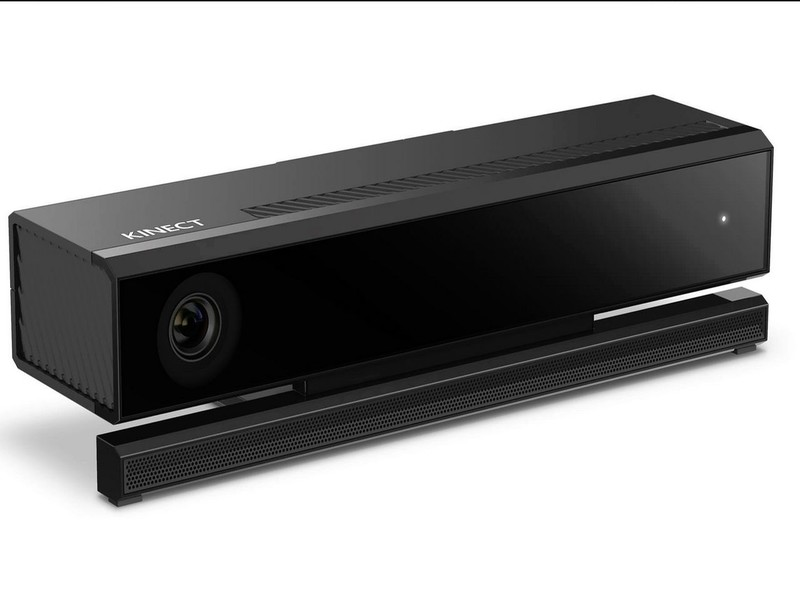
\includegraphics[width=0.3\columnwidth]{kinect}
    \caption[Microsoft Kinect]{Il Microsoft Kinect è un esempio di ToF Camera}
\end{figure}\\
I vantaggi maggiori sono, al contrario delle telecamere stereo, l'indipendenza dal contenuto della scena, e la maggiore rapidità poiché non richiede algoritmi particolari per il calcolo della disparità. \\
Tuttavia, la tecnologia non è esente da alcune limitazioni: 
\begin{itemize}
    \item Per superfici poco riflettenti o di colore scuro, il segnale di ritorno è debole, ciò risulta in misure poco accurate. 
    \item La limitata risoluzione spaziale non permette di ricavare una informazione dettagliata della geometria della scena.
    \item Il "multipath error" è un ulteriore problema che appare tipicamente vicino alle zone di incidenza tra le superfici. Esso è provocato dalla riflessione multipla del segnale luminoso prima di raggiungere il sensore \cite{rif1}. 
\end{itemize}

\section{Il Machine Learning}
Il machine learning, o apprendimento automatico, è una branca dell'informatica che fornisce ai computer la capacità di imparare ad eseguire un task da un certo insieme di dati di training, senza essere esplicitamente programmati a farlo. In sostanza, il machine learning esplora l'utilizzo di metodi matematico-computazionali per apprendere informazioni direttamente dai dati, senza modelli matematici ed equazioni predeterminate. Gli algoritmi di apprendimento automatico migliorano le loro prestazioni in modo "adattivo" mano a mano che gli "esempi" da cui apprendere aumentano. \par
I problemi che il machine learning punta a risolvere vengono classificati in tre categorie:
\begin{itemize}
    \item \textbf{Apprendimento supervisionato}: ogni istanza del set di esempi (training set) presenta gli input e i corrispondenti valori attesi in output. Questi esempi vengono presentati uno per volta alla macchina, il quale deve essere in grado di approssimare l'esatta natura della relazione presente tra l'input e il corrispondente output. L’obiettivo finale è dunque quello di insegnare al modello la capacità di predire correttamente i valori attesi su un set di istanze non presenti nel training set (test set). Questo scenario è quello trattato in questo lavoro di tesi.
    \item \textbf{Apprendimento non supervisionato}: al contrario dell'apprendimento supervisionato, gli output corrispondenti agli input forniti non sono conosciuti. All'algoritmo vengono presentati bensì numerosi dati dai quali la macchina deve estrarre le caratteristiche o i pattern nascosti. 
\end{itemize}
Esistono svariati approcci per la progettazione di sistemi di machine learning che vanno dagli alberi di decisione agli algoritmi genetici. La tecnica di interesse per il lavoro di questa tesi è quello basato sulle reti neurali artificiali.

\subsection{Reti neurali artificiali}
Le reti neurali artificiali (in inglese \textit{artificial neural network}, ANN) sono una classe di modelli matematici oggetto di numerosi studi. La loro importanza è derivata dal loro largo utilizzo in differenti ambiti e applicazioni. Da come suggerisce la parte "neurale" del nome, essi sono modelli che ricalcano il complesso funzionamento del sistema nervoso biologico. Le ANN sono composte da unità, chiamati neuroni, e le connessioni tra essi imitano il ruolo delle sinapsi.
\begin{figure}[ht]
    \centering
    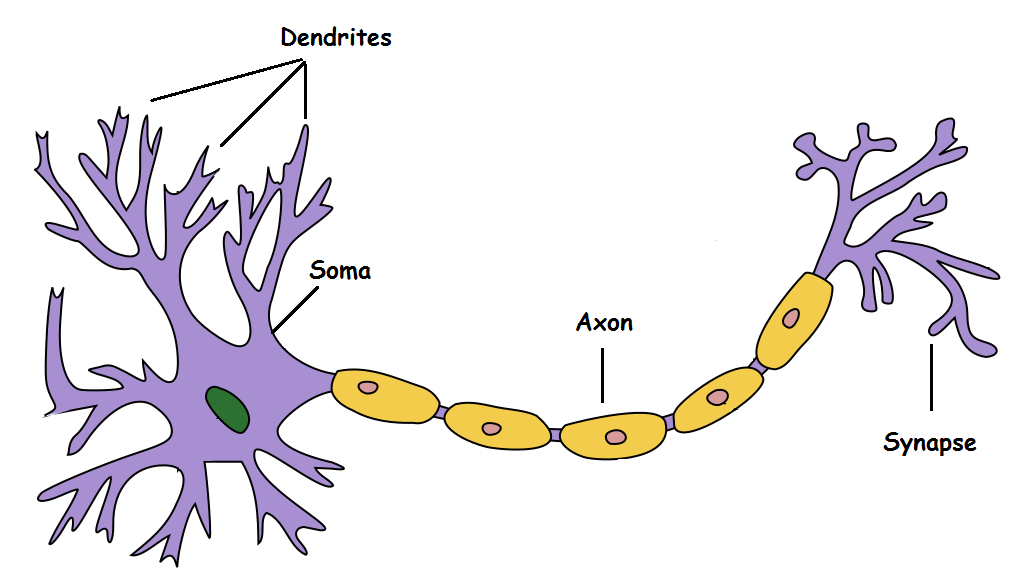
\includegraphics[width=0.5\columnwidth]{biological_neuron}
    \caption[Neurone biologico]{Neurone biologico \cite{maelfabien}}
\end{figure}
\paragraph{Percettrone}
Il più semplice modello dei neuroni artificiali è il \textit{percettrone}. 
\begin{figure}[ht]
    \centering
    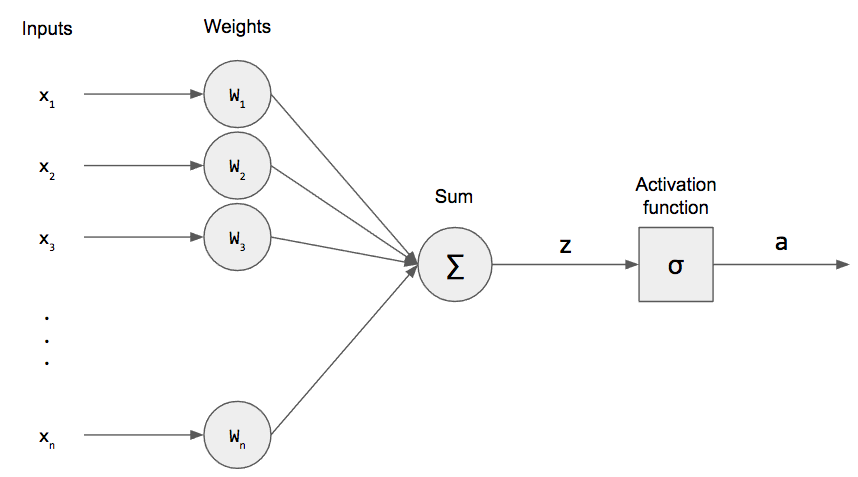
\includegraphics[width=0.5\columnwidth]{perceptron}
    \caption[Percettrone]{Schema di un percettrone \cite{pythonmachinelearning}}
\end{figure}
Esso prende in input un vettore di valori reali e ne effettua una combinazione lineare. Il risultato viene infine passato ad una funzione, detta funzione di attivazione, che restituisce l'output del neurone. Il modello complessivo può essere descritto dalla seguente formula: 
$$y=\sigma(\sum_{i} w_{i}x_{i}+b)$$
dove $w_{i}$ sono i pesi e b è un termine, detto bias, che viene aggiunto in seguito. Nel percettrone classico la funzione di attivazione $\sigma$ è una funzione a gradino, tuttavia sono numerose le alternative: tra i più comuni sono il sigmoide e il ReLU.
\paragraph{Deep Neural Network} 
Le reti neurali artificiali sono tipicamente organizzati in più strati, i nodi che la compongono sono suddivisi in tre macro-categorie. Abbiamo i nodi appartenenti allo strato di ingresso (input), i nodi appartenenti allo strato di uscita (output) e infine i nodi degli strati nascosti (hidden). L’architettura per strati è tipica delle reti neurali feed-forward. Tali reti sono caratterizzate dal fatto che l’attivazione dei nodi d’ingresso si propaga in avanti verso quelli dello strato (o degli strati) nascosto e da questi verso quelli dello strato di uscita.
\begin{figure}[ht]
    \centering
    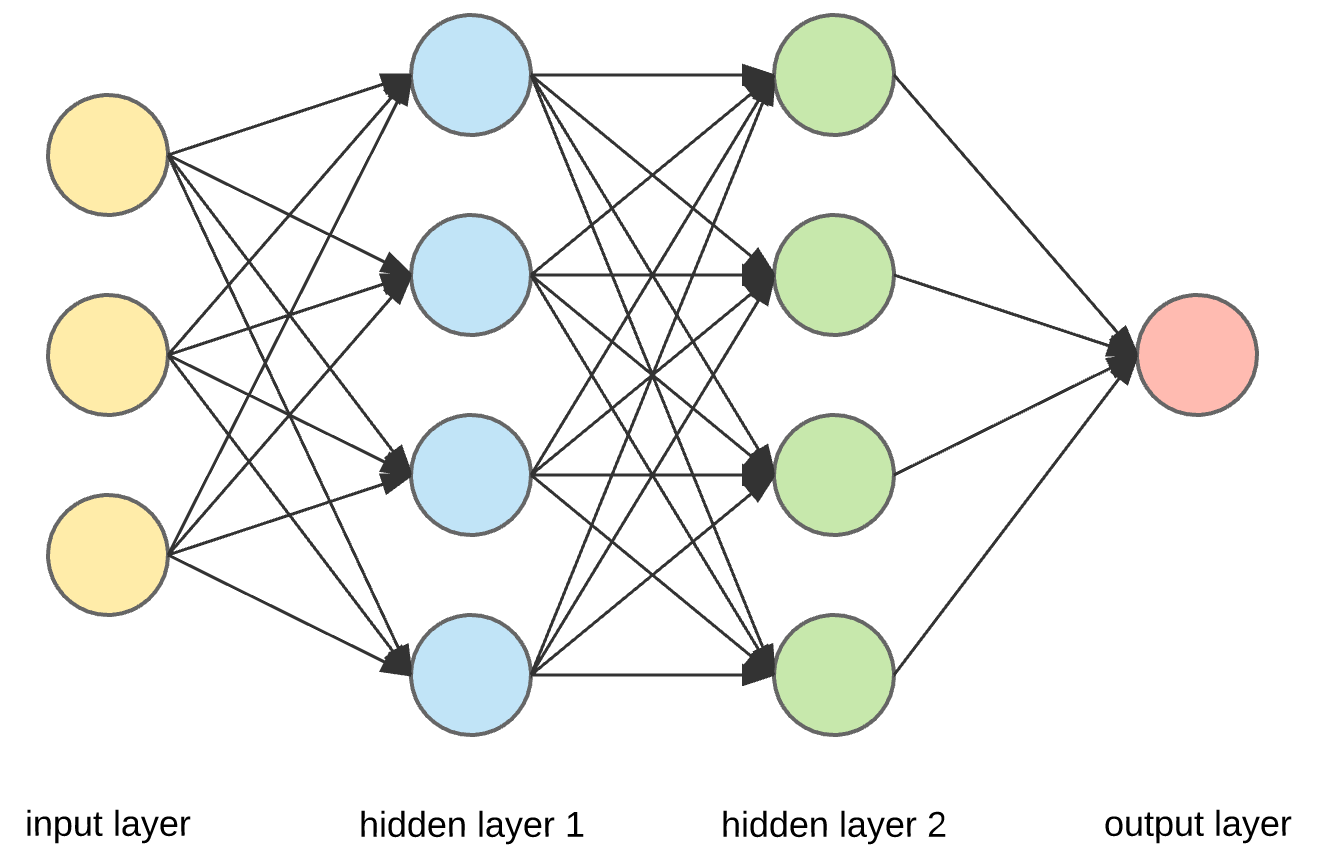
\includegraphics[width=0.5\columnwidth]{DNN}
    \caption[Deep Neural Network]{Rappresentazione di una rete neurale profonda \cite{ann}}
\end{figure}

\subsection{Reti neurali convoluzionali}
Le reti neurali visti fino ad ora sono composti da neuroni completamente interconnessi con ogni neurone del precedente e successivo strato. Ciò comporta un numero sproporzionato di pesi che devono essere gestiti all'aumentare degli strati e dei neuroni. Il problema diventa significativo dal punto di vista della memoria e del tempo di addestramento. Un altro svantaggio è l'\textit{overfitting}. Infatti, avere un grosso numero di parametri, implica che se il training set non è abbastanza grosso, la rete potrebbe imparare a discriminare perfettamente gli esempi del training set, però avere scarse prestazioni su dati nuovi.\par
Questi problemi sono stati affrontati efficacemente con le reti neurali convoluzionali (\textit{convolutional neural network}, CNN). Differentemente dalle tradizionali reti neurali, qui i neuroni sono connessi soltanto ad un sottoinsieme dei neuroni dello strato precedente, questa regione viene definita campo recettivo (\textit{receptive field}). Tale modello si ispira alla struttura della corteccia visiva del mondo animale. Nelle CNN approssimiamo la risposta di un singolo neurone agli stimoli del proprio campo recettivo attraverso una operazione di convoluzione.
\paragraph{Convoluzione} 
La convoluzione viene effettuata tra l'input di uno strato e uno o più filtri, detti anche \textit{kernel}. L'output della operazione di convoluzione è detta \textit{feature map}. Ci sono tante feature map quanti sono il numero di filtri utilizzati per elaborare gli input. 
\begin{figure}[ht]
    \centering
    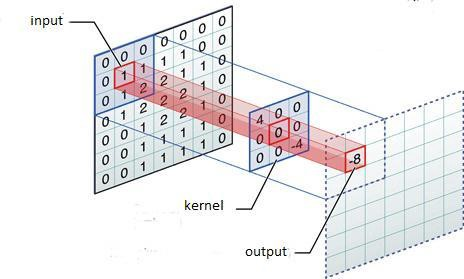
\includegraphics[width=0.5\columnwidth]{convolution}
    \caption[Esempio di convoluzione]{illustrazione della operazione di convoluzione con un filtro \cite{cnn}}
\end{figure}\\
Il principio di convoluzione è fondamentale: oltre a mantenere limitato il numero di parametri, esso fornisce una proprietà di invarianza alla traslazione. Di fatto, lo stesso filtro viene applicato su tutta l'immagine, ciò permette di rilevare una particolarità nell'immagine ovunque essa sia, indipendentemente dalla sua posizione. 
\paragraph{Funzioni di attivazione}
Analogamente alle reti neurali tradizionali, anche nelle CNN vengono usate le funzioni di attivazione. Questi vengono solitamente messi immediatamente dopo gli strati di convoluzione e hanno lo scopo di permettere alla rete l'apprendimento di funzioni non lineari. 
\begin{figure}[ht]
    \centering
    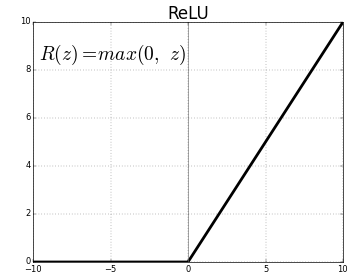
\includegraphics[width=0.3\columnwidth]{relu}
    \caption[Funzione di attivazione relu]{funzione di attivazione ReLU \cite{relu}}
\end{figure}
La funzione di attivazione più utilizzata in questo campo negli ultimi anni è il rettificatore lineare (\textit{Rectified Linear Unit}, ReLU). Questa, rispetto ad altre funzioni come la tangente iperbolica o la sigmoide, pone rimedio al problema del \textit{vanishing gradient}. Nelle reti molto profonde, infatti, le derivate sempre più in profondità possono diventare molto piccole, il che rende il training difficile. Essendo il gradiente della ReLU pari a 1 per i valori positivi e applicando la regola di derivazione a catena non si incorre in valori tendenti a zero. Ciò porta ad un processo di allenamento tendenzialmente più rapido.